\documentclass[CJKmath=true,10pt]{MyBook}


\usepackage{graphicx,float}
\usepackage{fontawesome5}
\usepackage[normalem]{ulem}
\usepackage{tikz}
\usetikzlibrary{arrows.meta, calc, patterns,angles,quotes}

\usepackage{siunitx}


\newcommand{\cgc}[3][]{
\begin{figure}[H]
\centering
\includegraphics[#1]{#2}
\caption{#3}
\end{figure}}

%设置一些字体
\usepackage{fontspec}
%\setCJKmainfont{Source Han Serif CN}
%[
%	Path=./fonts/hz/,
%	UprightFont = SourceHanSerifCN-Regular,
%	BoldFont = SourceHanSerifCN-Bold,
%	%ItalicFont = SourceHanSerifCN-Regular,
%	%BoldItalicFont = SourceHanSerifCN-Bold
%]
%\setCJKsansfont{Noto Sans CJK SC}
%[
%	Path=./fonts/hz/,
%	UprightFont = NotoSansCJKsc-Regular,
%	BoldFont = NotoSansCJKsc-Bold,
%	%ItalicFont = *-Regular,
%	%BoldItalicFont = *-Bold
%]
%\setCJKmonofont{Noto Sans Mono CJK SC}
%[
%UprightFont = *-Regular,
%BoldFont = *-Bold,
%AutoFakeSlant = 0.2
%]


% 定义 PowerShell 代码样式
\lstdefinelanguage{PowerShell}{
	keywords={Get-ChildItem, Rename-Item, -NewName, -replace, -WhatIf},
	morekeywords={Wait-Process, Get-Process},
	sensitive=false,
	morecomment=[l]{\#},
	morestring=[b]",
	morestring=[b]'
}

\lstset{
	language=PowerShell,
	basicstyle=\ttfamily\small,
	keywordstyle=\color{blue!80!black}\bfseries,
	stringstyle=\color{green!40!black},
	commentstyle=\color{gray}\itshape,
	frame=shadowbox,
	rulesepcolor=\color{gray!20},
	breaklines=true,
	showstringspaces=false,
	backgroundcolor=\color{gray!5}
}

\newcommand{\cuo}{\protect\textbf{\textcolor{red}{\ \faTimes\ \relax}}}
\newcommand{\dui}{\protect\textbf{\textcolor{green}{\ \faCheck\ \relax}}}

\begin{document}

%\frontmatter\tableofcontents
\mainmatter
%\setchapterimage{./images/055}
\setchapterimage{./images/bw}

\chapter{PowerShell的一些常用命令}
\section{核心理念}
PowerShell 的强大之处在于它处理的是\textbf{对象 (Objects)} 而非简单的文本字符串。
\begin{itemize}
	\item \textbf{输入}:不仅仅是文件名,而是包含属性(大小、时间、名称)的文件对象。
	\item \textbf{处理}:通过管道符流式处理每一个对象。
\end{itemize}

\section{命令详解}

\subsection{基本语法模板}
\begin{lstlisting}
Get-ChildItem <匹配模式>|Rename-Item -NewName {$_.Name -replace '正则查找', '替换内容'}
\end{lstlisting}

\subsection{参数逐步拆解}
\begin{enumerate}
	\item \ci{Get-ChildItem *.txt}:
	获取文件列表(类似 Linux 的 \ci{ls})。输出一系列文件对象。
	
	\item 管道符号“\ci{|}” :
	将左侧找到的每一个文件对象,逐个传递给右侧命令处理。
	
	\item \ci{Rename-Item}:
	执行重命名动作的命令。
	
	\item \ci{-NewName \{ ... \}}:
	接收一个\textbf{脚本块}。PowerShell 会对管道传来的\textbf{每一个}文件执行此代码,计算出新的名字。
	
	\item \textcolor{red}{\texttt{\$\_}} (当前对象):
	在脚本块中,\ci{\$\_} 代表“当前正在处理的这个文件”。
	\begin{itemize}
		\item \texttt{\$\_.Name}:获取完整文件名(如 \texttt{data.txt})。
	\end{itemize}
	
	\item \textbf{\texttt{-replace}} (操作符):
	语法:
	\begin{lstlisting}
'源' -replace '正则', '新内容'
	\end{lstlisting}
	\begin{itemize}
		\item 默认\textbf{不区分大小写}。
		\item 支持标准正则(如 \ci{^} 开头,\texttt{\$} 结尾)。
		\item 支持捕获组引用(如 \texttt{\$1})。
	\end{itemize}
\end{enumerate}

\section{实战场景与技巧}

\subsection{1. 安全模式 (强烈推荐)}
在正式执行前,务必添加 \texttt{-WhatIf} 参数进行预览,防止误操作。
\begin{lstlisting}
Get-ChildItem *.log | Rename-Item -NewName {$_.Name -replace 'old', 'new'} -WhatIf
\end{lstlisting}

\subsection{2. 使用捕获组调换顺序}
场景:将 \texttt{Part1\_Invoice.pdf} 改为 \texttt{Invoice\_Part1.pdf}。
\begin{lstlisting}
Get-ChildItem *.pdf | Rename-Item -NewName {$_.Name -replace '^(Part\d+)_(.+)\.pdf$','$2_$1.pdf'}
\end{lstlisting}
\textit{注:\texttt{\$1} 和 \texttt{\$2} 对应正则表达式中括号捕获的内容。}

\subsection{3. 仅操作文件名 (保留扩展名)}
如果担心误改扩展名,可以使用 \texttt{\$\_.BaseName} 仅获取主文件名。
\begin{lstlisting}
# 仅给文件名前加 Backup_,不影响后续扩展名
Get-ChildItem * | Rename-Item -NewName { 'Backup_' + $_.Name }
\end{lstlisting}

\section{总结公式}
\begin{tcolorbox}[colback=blue!5!white,colframe=blue!75!black,title=记忆口诀]
	Let (获取列表) $\rightarrow$ Pipe (管道传入) $\rightarrow$ Rename (重命名命令) $\rightarrow$ Script (计算新名)
\end{tcolorbox}

\chapter{传送带专题}
\section{传送带问题一般分析方法}
%\includegraphics{./pics/1.png}
\begin{figure}[H]
\centering
\begin{tikzpicture}[>=Stealth, scale=1]
    % === Left: Conveyor Belt Diagram ===
    \begin{scope}
        \def\R{0.6} % Pulley radius
        \def\L{5.0}   % Distance between pulley centers
        
        % Pulleys
        \filldraw[fill=gray!20] (0,0) circle (\R);
        \filldraw[fill=gray!20] (\L,0) circle (\R);
        \draw[fill=black] (0,0) circle (0.05);
        \draw[fill=black] (\L,0) circle (0.05);
        
        % Belt
        \draw[thick] (0,\R) -- (\L,\R);
        \draw[thick] (0,-\R) -- (\L,-\R);
        
        % Rotation arrow (clockwise on right pulley)
        \draw[->, thick, black] (\L+\R-0.25, \R-0.25) arc (45:-90:0.4);
        
        % Block (placed on left side)
        \coordinate (BlockPos) at (0.4, \R+0.05);
        \draw[fill=blue!30] (BlockPos) rectangle ++(0.8, 0.5);
        \node at ($(BlockPos)+(0.4, 0.25)$) {$m$};
        
        % Velocity vectors
        % v0 (Block)
        \draw[->, thick, red] ($(BlockPos)+(\R/4, 0.05)$) -- ++(1.0, 0) node[right] {$\mu mg$};
        % v (Belt)
        \draw[->, thick, black] (\L/3, \R-0.4) -- ++(1.2, 0) node[right] {$v_0$};
        
        % Labels
        \node[below] at (0,-\R) {$A$};
        \node[below] at (\L,-\R) {$B$};
        
        \node[below, align=center] at (\L/2, -1.0) {传送带足够长};
    \end{scope}

    % === Right: v-t Graph ===
    \begin{scope}[shift={(8,-1)}]
    	\coordinate (O) at (0, 0);
    	\coordinate (TC) at (2, 1.5);
    	\coordinate (T1) at (2, 0);
    	\coordinate (V0) at (0, 1.5);
        
        

        % Axes
        \draw[thick,->] (-0.5, 0) -- (4, 0) node[below] {$t$};
        \draw[thick,->] (0, -0.5) -- (0, 2.5) node[left] {$v$};
        \node[below left] at (O) {$O$};
        
        % Belt velocity v (dashed line)
        \draw[dashed, red, thick] (V0) -- (3.5, 1.5) node[right] {$v_0$};
        \node[left, red] at (0, 1.5) {$v_0$};
        
        % Block velocity behavior: v0 -> v then constant
        % Coordinate definitions

       
        
        
        % Curve
        \draw[blue, thick] (O) -- (TC);
        
        % TC mark
        \draw[dashed] (TC) -- (2, 0) node[below] {$t_1$};
        
        % Fill the area enclosed by O, TC, V0
        \fill[pattern=horizontal lines, pattern color=red] (O) -- (TC) -- (V0) -- cycle;
        \fill[pattern=vertical lines, pattern color=blue] (O) -- (T1) -- (TC) -- cycle;
    \end{scope}
\end{tikzpicture}
\caption{水平红色三角形区域面积表示相对位移,蓝色竖直三角形区域面积表示对地位移。}
\end{figure}
对于水平传送带,只要物块速度比传送带慢,就一定加速。如果传送带慢,物块有初速度并且比传送带快,那么一定减。最终两者会达到共速。
\begin{figure}[H]\centering
    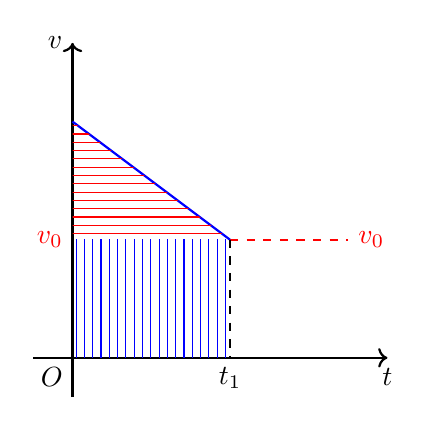
\begin{tikzpicture}
	\coordinate (O) at (0, 0);
	\coordinate (TC) at (2, 1.5);
	\coordinate (T1) at (2, 0);
	\coordinate (V0) at (0, 1.5);
	\coordinate (V1) at (0,3);
	
	
	
	% Axes
	\draw[thick,->] (-0.5, 0) -- (4, 0) node[below] {$t$};
	\draw[thick,->] (0, -0.5) -- (0, 4) node[left] {$v$};
	\node[below left] at (O) {$O$};
	
	% Belt velocity v (dashed line)
	\draw[dashed, red, thick] (TC) -- (3.5, 1.5) node[right] {$v_0$};
	\node[left, red] at (0, 1.5) {$v_0$};
	
	% Block velocity behavior: v0 -> v then constant
	% Coordinate definitions
	
	
	
	
	% Curve
	\draw[blue, thick] (V1) -- (TC);
	
	% TC mark
	\draw[dashed] (TC) -- (2, 0) node[below] {$t_1$};
	
	% Fill the area enclosed by O, TC, V0
	\fill[pattern=horizontal lines, pattern color=red] (V0) -- (TC) -- (V1) -- cycle;
	\fill[pattern=vertical lines, pattern color=blue] (O) -- (T1) -- (TC) -- (V0)--cycle;
\end{tikzpicture}
	\caption{物块比传送带快的情况}
\end{figure}
\begin{itemize}
	\item \textbf{同向}:依据物块初速度和传送带的速度大小\textbf{快减慢加}。
	\item \textbf{反向}则一定减速,减速到0后再加速,然后共速\footnote{此种情况,可以结合竖直上抛运动,两者极为相似,也称\textbf{反上抛}。}。
\end{itemize}

在\textbf{水平}传送带运动中,滑动摩擦力提供的最大加速度$a=\mu g$。如果传送带是匀速的,在共速后,不需要外力,只需要惯性就可以维持物体和传送带一起运动,因此此时的滑动摩擦力一定够用。

如果传送带有加速度,则情况变得复杂了,物体放上传送带时就需要判断最大静摩擦力提供的加速度$\mu g$能否追上传送带的加速度。通常使用$VT图$直接判断,如果$\mu g \ge a_{传送带}$,其实就变成了追击问题;如果小,更简单,永远不能共速,也就是物体一直在传送带上\textbf{打滑}。$a$大$\mu g$小必打滑。

对于水平传送带有加速并且$\mu g \ge a_{传送带}$,在共速后,因为摩擦力可以提供足够的加速度,因此两者一直共速,即物体也和传送带有同样的加速度(物体的加速度不可能超过传送带的加速度)。

对于倾斜传送带,$a_{斜滑}=g\cdot\sin\theta \pm \mu\cdot g\cdot\cos\theta$。如果物体\textbf{相对传送带}沿斜面向上滑,重力在斜面的分量和摩擦力一致,取“$+$”,否则取“$-$”。

\section{有限长传送带}
\begin{figure}[H]
	\centering
	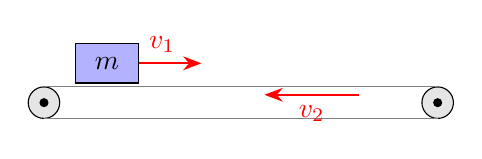
\begin{tikzpicture}[>=Stealth, scale=1]
			\def\R{0.2} % Pulley radius
			\def\L{5.0}   % Distance between pulley centers
			
			% Pulleys
			\filldraw[fill=gray!20] (0,0) circle (\R);
			\filldraw[fill=gray!20] (\L,0) circle (\R);
			\draw[fill=black] (0,0) circle (0.05);
			\draw[fill=black] (\L,0) circle (0.05);
			
			% Belt
			\draw[gray] (0,\R) -- (\L,\R);
			\draw[gray] (0,-\R) -- (\L,-\R);
			
			
			% Block (placed on left side)
			\coordinate (BlockPos) at (0.4, \R+0.05);	
			% Velocity vectors
			% v0 (Block)
			\draw[->, thick, red] ($(BlockPos)+(0.6, 0.25)$) -- ++(1.0, 0) node[above,midway] {$v_1$};
			\draw[fill=blue!30] (BlockPos) rectangle ++(0.8, 0.5);
			\node at ($(BlockPos)+(0.4, 0.25)$) {$m$};
			
		
			% v (Belt)
			\draw[->, thick, red] (4, 0.1) -- ++(-1.2, 0) node[below,midway] {$v_2$};
			
			

	\end{tikzpicture}
	\caption{有限长传送带}
\end{figure}	
\subsection{$V_0$与$V_{带}$反向}
\subsubsection{冲出(传送带不够长)}
最简单情况:传送带没有足够长,物块直接冲出传送带。冲出的原因:物块在减速到0之前(对地最大位移),对地位移已经超出传送带长度$L$。如果把减速到0的对地位移记做$X_{减}$,则:\(X_{减}=\dfrac{V_1^2}{2\mu g}\)。如果$>L$则冲出,冲出时速度$V'=\sqrt{V_1^2-2\mu gL}$。像这种不涉及时间的,用速方差公式简单。
\begin{figure}[H]
	\centering
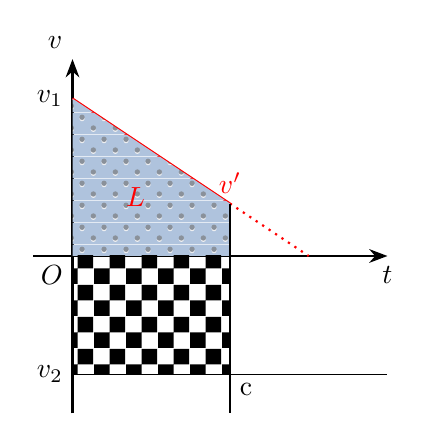
\begin{tikzpicture}[>=Stealth]
	\coordinate (O) at (0, 0);
	\coordinate (v1) at (0,2);
	\coordinate (v2) at (0,-1.5);
	\coordinate (vt) at(3,0);
	\coordinate (stop) at(2,2/3);
	\coordinate (st)at(2,0);
	\coordinate (c)at(2,-1.5);
	% Axes
	\draw[thick,->] (-0.5, 0) -- (4, 0) node[below] {$t$};
	\draw[thick,->] (0, -2) -- (0, 2.5) node[above left] {$v$};
	\node[below left] at (O) {$O$};
	
	\draw(v2) -- ++(4, 0);
	\draw[thick, red] (v1) -- (stop) node[below,midway] {$v_2$};
	\draw[thick,dotted, red] (stop) -- (vt);
	\path[pattern=crosshatch dots light steel blue] (O)--(st)--(stop)--(v1)--cycle;
	\node[left] at(v1){$v_1$};
	\node[left] at(v2){$v_2$};
	\draw(stop)--(st)--++(0,-2);
	\node[red] at(0.8,0.75){$L$};
	\node[red,above]at(stop){$v'$};
	\path[red,pattern=checkerboard](O)--(st)--(c)node[below right,black]{c}--(v2)--cycle;
%	% Belt velocity v (dashed line)
%	\draw[dashed, red, thick] (V0) -- (3.5, 1.5) node[right] {$v_0$};
%	\node[left, red] at (0, 1.5) {$v_0$};
%	
%	% Block velocity behavior: v0 -> v then constant
%	% Coordinate definitions
%	
%	
%	
%	
%	% Curve
%	\draw[blue, thick] (O) -- (TC);
%	
%	% TC mark
%	\draw[dashed] (TC) -- (2, 0) node[below] {$t_1$};
%	
%	% Fill the area enclosed by O, TC, V0
%	\fill[pattern=horizontal lines, pattern color=red] (O) -- (TC) -- (V0) -- cycle;
%	\fill[pattern=vertical lines, pattern color=blue] (O) -- (T1) -- (TC) -- cycle;
\end{tikzpicture}
	\caption{$v'$是滑下时物块速度,L是对地位移,也是传送带长度,棋盘格围成的面积是传送带位移}
\end{figure}
梯形$v_1v'cv_2$围成的面积是物块相对传送带的位移,两者是加法。
\subsubsection{折返(传送带足够长)}
当物块速度为0时,对地位移$\le L$时,即传送带\emph{足够长},会发生折返,类似上抛运动。

\subsubsection{半折返}
对于$v_1>v_2$,则到达速度0点,然后折返,折返后速度最大只能达到$v_2$:
\begin{figure}[H]
	\centering
	\begin{tikzpicture}[>=Stealth]
		\coordinate (O) at (0, 0);
		\coordinate (v1) at (0,2);
		\coordinate (v2) at (0,-1);
		\coordinate (vc)at(3,-1); %交点
		\coordinate (v0)at(2,2); %0速度点
		% Axes
		\draw[thick,->] (-0.5, 0) -- (4, 0) node[below] {$t$};
		\draw[thick,->] (0, -2) -- (0, 2.5) node[above left] {$v$};
		\node[below left] at (O) {$O$};
		\draw(v1)node[left]{$v_1$}--(vc)node[below right]{共速}--++(1,0);
		\draw[dotted](v2)node[left]{$v_2$} -- (vc);
		\node at(.5,1){$X_{max}$};
		%	% Belt velocity v (dashed line)
		%	\draw[dashed, red, thick] (V0) -- (3.5, 1.5) node[right] {$v_0$};
		%	\node[left, red] at (0, 1.5) {$v_0$};
		%	
		%	% Block velocity behavior: v0 -> v then constant
		%	% Coordinate definitions
		%	
		%	
		%	
		%	
		%	% Curve
		%	\draw[blue, thick] (O) -- (TC);
		%	
		%	% TC mark
		%	\draw[dashed] (TC) -- (2, 0) node[below] {$t_1$};
		%	
		%	% Fill the area enclosed by O, TC, V0
		%	\fill[pattern=horizontal lines, pattern color=red] (O) -- (TC) -- (V0) -- cycle;
		%	\fill[pattern=vertical lines, pattern color=blue] (O) -- (T1) -- (TC) -- cycle;
	\end{tikzpicture}
	\caption{$v_1>v_2$时}
\end{figure}
此时,物块回到出发点所用时间
\[ t_总=\dfrac{v_1-v_2}{\mu g}+\dfrac{v_1^2-v_2^2}{2v_2\mu g}\]
此公式可以由图得出,并且注意$v_1,v_2$异号,其实就是绝对值加。


\subsection{$V_0$与$V_{带}$同向}
\subsubsection{L不够长}
一定\textbf{全程加速度不变},因为达到共速前已经冲出传送带了。
\subsection{感想}
其实各种情况都太复杂了,可以简化成:物块在光滑的水平面运动,在其速度达到传送带的速度之前,持续受到恒力$\mu mg$的作用。也可以按竖直上(初速度与传送带异向)下(初速度与传送带同向)抛,自由落体(初速度为0)来计算,只是$a=\mu g$。

传送带模型之所以简单,就是因为加速度不变。
\end{document}